\chapter{Introduction}
\label{ch:introduction}

\epigraph{All models are wrong, but some are useful.}{--- George E.P. Box}

\section{Renal Cell Carcinoma: Clinical Significance}
\label{sec:intro_epidemiology}

\lettrine[lines=2]{R}{enal cell carcinoma} (RCC) affects 400,000 people annually worldwide, with metastatic disease carrying a five-year survival rate of approximately 15\%~\cite{santoni2024}. Clear cell RCC (ccRCC) constitutes 70--80\% of cases and is characterized by \emph{von Hippel--Lindau} (\emph{VHL}) mutations leading to vascular endothelial growth factor (VEGF) overexpression---making it both a target for anti-angiogenic therapies and one of the tumors most responsive to immunotherapy due to its high immunogenicity~\cite{pardoll2012}. Despite the success of checkpoint immunotherapy in reshaping the treatment landscape, approximately 40\% of advanced RCC patients do not respond to first-line treatment, and there are currently no validated biomarkers that reliably predict which patients will benefit from immune checkpoint inhibitors (ICI) versus tyrosine kinase inhibitors (TKI) versus combination therapy---underscoring an urgent unmet need for predictive tools that can stratify patients and guide therapeutic decisions. Figure~\ref{fig:rcc_epidemiology} summarizes the global incidence rates, sex distribution, and stage-dependent survival patterns that motivate the sex-stratified approach adopted in this work.

\begin{figure}[htbp]
\centering
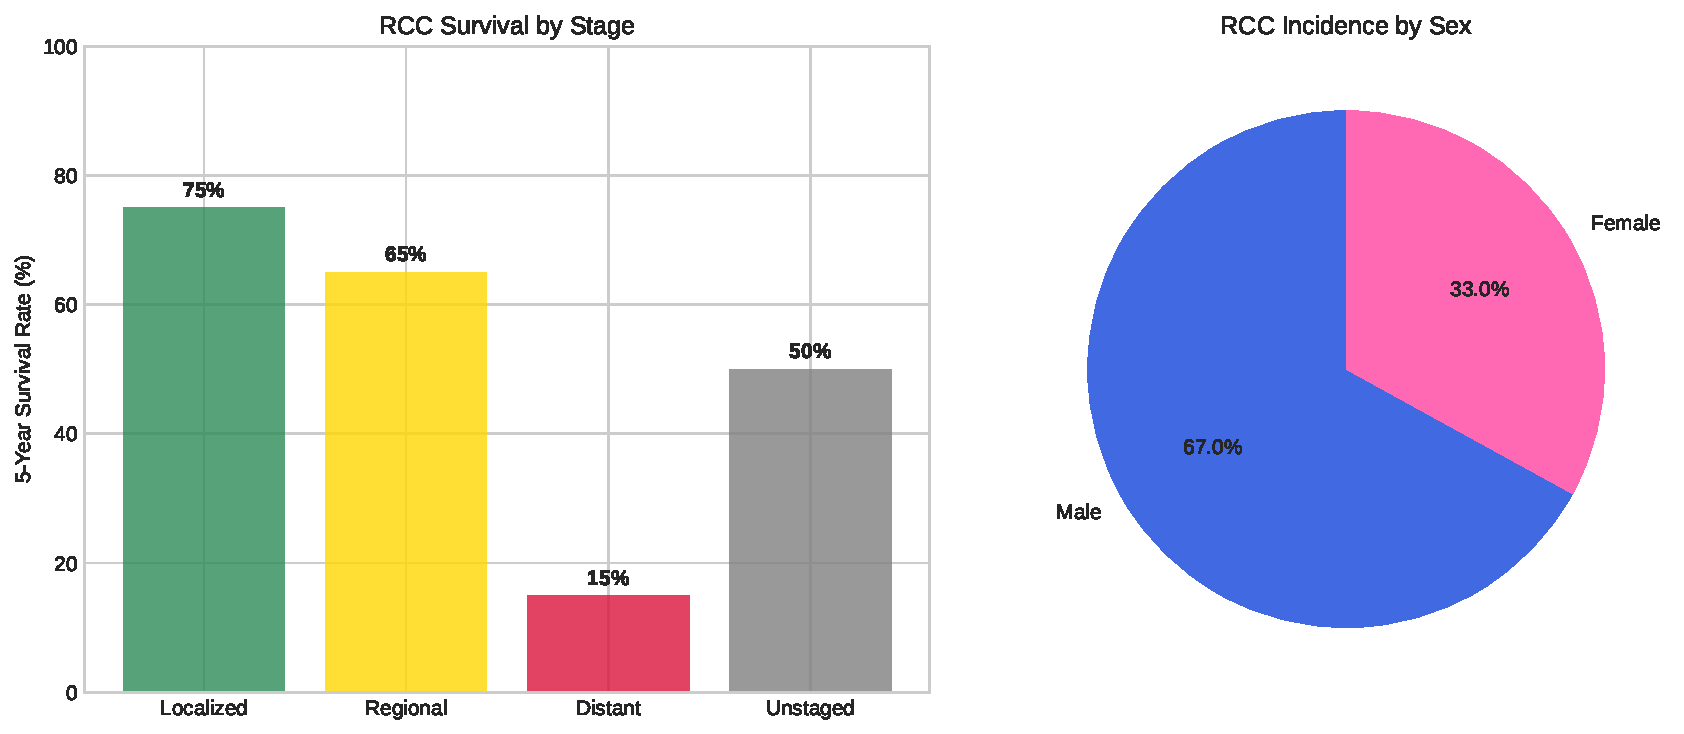
\includegraphics[width=0.85\textwidth]{figures/rcc_epidemiology.pdf}
\caption{Renal cell carcinoma epidemiology data showing global incidence rates, sex distribution, and stage-dependent survival curves. The pronounced male predominance (2:1 ratio) and stage-dependent survival patterns motivate the sex-stratified modeling approach and clinical calibration used in this work.}
\label{fig:rcc_epidemiology}
\end{figure}

\section{The Tumor Microenvironment and Sex Differences}
\label{sec:intro_tme}

The tumor microenvironment (TME) is a complex, spatially heterogeneous ecosystem encompassing tumor cells, immune cells (cytotoxic T lymphocytes (CTLs), Th1/Th2, Tregs, DCs, M1/M2 macrophages, NK cells), vasculature, and signaling molecules. The bidirectional interactions between these components create nonlinear dynamics where immune cells can kill tumors but tumors can also co-opt immune responses to establish immunosuppressive niches~\cite{hanahan2011}.

Critically, the \emph{spatial organization} of these cellular populations---not merely their relative abundances---determines clinical outcomes. Tumors classified as ``immune-inflamed,'' in which CTLs infiltrate deep into the tumor parenchyma, respond markedly better to checkpoint immunotherapy than ``immune-excluded'' tumors, where effector cells accumulate at the tumor periphery but fail to penetrate the core, or ``immune-desert'' tumors, which lack significant immune infiltration altogether~\cite{chen2017}. This spatial heterogeneity arises from physical barriers such as aberrant vasculature and dense extracellular matrix, as well as from chemokine gradients and metabolic competition that shape immune cell trafficking. Traditional ordinary differential equation (ODE) models, which represent cell populations as well-mixed compartments, cannot capture these spatially mediated phenomena: they cannot distinguish between a thousand T~cells uniformly distributed throughout a tumor and a thousand T~cells trapped at its margin---two configurations with profoundly different therapeutic implications. Agent-based models, by contrast, represent each cell as a discrete entity occupying a specific spatial position, making them a natural formalism for studying how tumor topology governs immune access and treatment efficacy.

RCC exhibits a pronounced sex bias, with males showing approximately twice the incidence of females across virtually all populations studied~\cite{znaor2015}. This disparity extends beyond incidence: male patients tend to present with higher-stage disease and experience worse stage-for-stage survival, suggesting that sex-linked biological factors influence progression and treatment response. Estrogen shows biphasic effects on immunity---enhancing innate and adaptive responses at physiological concentrations but promoting immunosuppression at higher levels---while testosterone generally suppresses immune responses and promotes immune evasion. Beyond hormonal effects, X-chromosome--linked immune genes (including \emph{TLR7}, \emph{FOXP3}, and \emph{CD40L}) may contribute to stronger baseline immune surveillance in females. Despite these well-documented differences, most RCC clinical trials have not stratified outcomes by sex. The ARON-1 clinical study~\cite{santoni2024} directly addresses this gap by investigating sex-dependent treatment responses in advanced ccRCC, comparing ICI, TKI, and combination therapy across male and female cohorts, and provides the primary clinical benchmark against which the present model is calibrated.

\section{Motivation for Computational Modeling}
\label{sec:intro_motivation}

The complexity of the RCC tumor microenvironment---with heterogeneous cell populations, spatial organization, stochastic interactions, metabolic competition, and hormonal modulation---presents a challenge that no single experimental or analytical approach can fully address. Clinical trials are expensive, time-consuming, and limited in the treatment combinations and patient subpopulations they can explore. Computational modeling offers a complementary path by enabling \emph{in silico} experimentation with thousands of virtual patients, systematic exploration of inaccessible parameter spaces, algorithmic treatment optimization, and generation of mechanistic hypotheses for experimental testing. In RCC specifically, such models may address the biomarker gap by simulating how patient-specific variables interact to determine treatment response, identifying subpopulations for whom particular therapies are most likely to succeed.

Previous work by Merelli et al.~\cite{merelli2021} demonstrated the feasibility of agent-based RCC modeling using the Mesa framework, reproducing qualitative features of RCC progression on a two-dimensional lattice with simplified immune cell types. However, their model was limited to single-process execution, two-dimensional geometry, and lacked metabolic competition, sex hormone modulation, or clinical calibration. The present work extends that foundation in five directions: porting to Repast4Py for MPI-based parallelism, adding a continuous three-dimensional glucose field based on Fick's diffusion, introducing a 16-gene DNA system with codon-level mutation mechanics, incorporating sex hormone modulation of immune responses, and calibrating against ARON-1 clinical trial data using Bayesian optimization. Figure~\ref{fig:conceptual_overview} provides a high-level overview of this modeling approach.

\begin{figure}[htbp]
\centering
\adjustbox{max width=0.85\textwidth, max height=0.7\textheight}{% Conceptual Overview Diagram for Chapter 1
\begin{tikzpicture}[scale=0.8, every node/.style={scale=0.8}]

% Define professional color palette
\definecolor{patient}{RGB}{67, 56, 202}       % Indigo
\definecolor{tumor}{RGB}{220,20,60}          % Crimson
\definecolor{immune}{RGB}{16, 185, 129}      % Emerald  
\definecolor{treatment}{RGB}{245, 158, 11}   % Amber
\definecolor{prediction}{RGB}{138,43,226}    % Purple
\definecolor{validation}{RGB}{249, 115, 22}  % Orange

% Patient input
\node[draw, rounded corners=3pt, fill=patient!20, text width=3cm, text centered, drop shadow] (patient) at (0,8) {
    \textbf{Patient Input}\\
    • Sex (M/F)\\
    • BMI\\
    • Tumor Volume\\
    • Mutation Profile
};

% Simulation layer
\node[draw, rounded corners=3pt, fill=immune!10, text width=12cm, text centered, minimum height=6cm, drop shadow] (simulation) at (6,5) {
    \textbf{Agent-Based Simulation}\\
    \vspace{0.3cm}
    \begin{minipage}{11cm}
        18 Agent Types • 3D Spatial Grid • Glucose Field\\
        MPI Parallel Execution • Repast4Py Framework
    \end{minipage}
};

% Tumor cells
\node[draw, circle, fill=tumor, text=white, drop shadow] (tumor1) at (3,6) {TC};
\node[draw, circle, fill=tumor, text=white, drop shadow] (tumor2) at (3.5,5.5) {TC};
\node[draw, circle, fill=tumor, text=white, drop shadow] (tumor3) at (2.5,5.5) {TC};

% Immune cells
\node[draw, circle, fill=immune, text=white, drop shadow] (tcell1) at (5,6.5) {CTL};
\node[draw, circle, fill=immune, text=white, drop shadow] (tcell2) at (5.5,6) {NK};
\node[draw, circle, fill=immune, text=white, drop shadow] (macro) at (4.5,5.5) {M1};
\node[draw, circle, fill=immune, text=white, drop shadow] (dc) at (6,5.5) {DC};

% Blood vessels
\draw[line width=3pt, bloodvessel] (1.5,4.5) -- (8.5,4.5);
\node[bloodvessel] at (9,4.5) {Blood Vessels};

% Glucose gradient
\fill[glucose!30] (2,3.5) ellipse (1.5 and 0.5);
\fill[glucose!60] (4,3.5) ellipse (1 and 0.3);
\fill[glucose!90] (6,3.5) ellipse (0.8 and 0.2);
\node[glucose] at (8,3.5) {Glucose Field};

% Treatment input
\node[draw, rounded corners=3pt, fill=treatment!20, text width=3cm, text centered, drop shadow] (treatment_input) at (0,2) {
    \textbf{Treatment}\\
    • ICI\\
    • TKI\\
    • Combination\\
    • None
};

% Outcomes
\node[draw, rounded corners=3pt, fill=prediction!20, text width=4cm, text centered, drop shadow] (outcomes) at (12,8) {
    \textbf{Predicted Outcomes}\\
    • Survival Probability\\
    • Treatment Response\\
    • Optimal Therapy\\
    • Biomarker Profiles
};

% ARON-1 validation
\node[draw, rounded corners=3pt, fill=validation!20, text width=3cm, text centered, drop shadow] (aron1) at (12,2) {
    \textbf{ARON-1 Study}\\
    Clinical Data\\
    Validation\\
    Calibration
};

% Arrows with professional styling
\draw[-{Stealth[length=3mm]}, thick, patient] (patient) -- (simulation);
\draw[-{Stealth[length=3mm]}, thick, treatment] (treatment_input) -- (simulation);
\draw[-{Stealth[length=3mm]}, thick, prediction] (simulation) -- (outcomes);
\draw[-{Stealth[length=3mm]}, thick, dashed, validation] (aron1) -- (simulation);

% Add interaction arrows between agents
\draw[-{Stealth[length=2mm]}, tumor, thick] (tcell1) -- (tumor1);
\draw[-{Stealth[length=2mm]}, tumor, thick] (tcell2) -- (tumor2);
\draw[-{Stealth[length=2mm]}, immune, dashed] (dc) -- (tcell1);

% Add title
\node[text width=14cm, text centered] at (6,10) {
    \Large\textbf{RCC Agent-Based Model: From Patient to Prediction}
};

\end{tikzpicture}}
\caption{Conceptual overview of the RCC agent-based modeling approach.}
\label{fig:conceptual_overview}
\end{figure}

\section{Agent-Based Modeling Approach}
\label{sec:intro_abm}

Agent-based modeling (ABM) is a computational paradigm in which a system is represented as a collection of autonomous entities---agents---that interact with each other and their environment according to defined rules, with macroscopic behavior emerging from the aggregate of local interactions. ABM is particularly well suited to the tumor microenvironment because each agent can carry its own state---a unique genome, activation level, spatial position, and accumulated neighbor effects---providing natural representation of cellular heterogeneity. Agents occupy positions in a 3D grid and interact with their local neighborhood, capturing spatial phenomena such as immune-excluded regions, vascular networks, and glucose gradients. Biological processes like division, apoptosis, and immune recognition are inherently probabilistic, and ABM naturally incorporates this stochasticity at the individual level, allowing complex phenomena such as immune evasion and treatment resistance to emerge from simple local rules without explicit programming.

The choice of Repast4Py~\cite{repast4py} as the simulation framework is motivated by its support for MPI-based parallel execution, enabling the model to scale to larger grid sizes and agent populations than single-process frameworks such as Mesa~\cite{mesa}. Repast4Py provides core abstractions---\texttt{SharedContext}, \texttt{SharedGrid}, and MPI-aware scheduling---that distribute agents across processes while maintaining consistent spatial queries and inter-agent communication.

\section{Project Objectives}
\label{sec:intro_objectives}

This work pursues four principal objectives. First, the existing Mesa model is ported to Repast4Py for MPI parallelism, restructuring the agent hierarchy, spatial indexing, and scheduling while preserving all 18 agent types and their interaction logic. Second, a novel continuous 3D glucose concentration field is overlaid on the agent grid, where blood vessels inject glucose that diffuses via Fick's law and is consumed by all cell types at metabolically appropriate rates, introducing 8 new parameters governing glucose dynamics. Third, the model's predictions are validated against ARON-1 clinical trial data with particular attention to sex-stratified treatment responses. Fourth, an Optuna-based Bayesian optimization pipeline searches the parameter space for configurations reproducing clinical observations.

\section{Report Structure}
\label{sec:intro_structure}

The report proceeds from theoretical background (Chapter~\ref{ch:theoretical_background}) through model architecture and biological subsystems (Chapters~\ref{ch:model_description}--\ref{ch:biological-subsystems}), treatment mechanisms (Chapter~\ref{ch:treatment}), implementation details (Chapter~\ref{ch:implementation}), and parameter optimization (Chapter~\ref{ch:parameters}), before presenting simulation results and validation (Chapter~\ref{ch:simulation-results}) and concluding with future directions (Chapter~\ref{ch:conclusion}).
